
A key aspect of RPM is the establishment and maintenance of providers' awareness of their patient’s condition and risk during home care.
Medical use and testing of \phware for this purpose will require design of an end-to-end system that must implement appropriate policy for risk awareness for COVID-19 patients during home care, and for transitions to-and-from their different levels of care.
We call this CWP \emph{actionable risk awareness} and the policy is adapted from \emph{NIH COVID-19 Treatment Guidelines} by the U.S. National Institute of Health \cite{NIH}.
The \emph{Guidelines} cover five levels of COVID-19 severity and appropriate treatments for each level.
The CWP represents the medical problem that must be solved by system designs for vital signs RPM that aim to implement the Guidelines.
They are summarized and represented here as the finite state machine in \figref{fig:cwp}.

The state machine is composed of the relevant states mild/presymptomic patients can occupy, their associated risks, and transition conditions among them. The actions for appropriate care are responses to physiological events. This specification of a set of transformations on a complex object of work provides clarity, rigor and technical neutrality for \emph{actionable risk awareness} to be shared by the activities of people and computing in a distributed cognitive system.

In the initial state of \figref{fig:cwp} all patients have tested positive for COVID-19. If exams find their severity needs are greater than home care allows those patients follow the arc labeled letter-\textbf{B}  (\emph{sevNeed $>$homeCare}) and are ordered to ambulatory care or hospital admission.
The remaining focus of Fig.1 is on patients with initial exam findings that are pre/asymptomatic or have mild symptoms without comorbidities (letter-\textbf{A}).
They are ordered to home care with RPM of vitals because treatment there is equal-to-or-greater-than their severity level needs (\emph{$sevNeed \le homeCare$}).
In the state \emph{pt n appropriate home care} their vitals are measured at provider-ordered times ordered for analysis and RPM to begin \emph{actionable risk awareness}.

Patients remain in home care until either meeting discharge criteria (letter-\textbf{C}); or the trend of their condition or home care deteriorates \emph{trndSevNeed $>$homeCare} (letter-\textbf{D}) putting them in the state \emph{pt at elevated risk in home care}.
Patients must not remain in this state because it has a direct path of fatality (letter-\textbf{G}).
A near-future exam must determine if they are ordered to clinical care (letter-\textbf{E}) or whether they can be restored to \emph{$sevNeeds\le homeCare$} with increased RPM or medication for new symptoms (letter-\textbf{F}).
If ordered to ambulatory care or hospital care patients can be discharged \textbf{C}, or expire \textbf{G}.

The \emph{NIH Guidelines} are an authoritative source, but their translation to a finite state diagram needed review for validation. 
Early versions of Fig.1 served as a story board that allowed critiquing by doctors. 
One critique led us to add more content to letter-A about the types of home care.  
For another, we added the primary care provider's exam (PCP exam) as part of discharge orders.

Importantly, the CWP is independent of any technology beyond vital signs measuring, and could be satisfied by a variety of designs.  
As presented next, this technical independence allows the CWP's logical content to serve as the criterial property for model-checking to verify the integrated design.

\begin{figure}[t]
  \begin{center}
    \begin{tabular}{c}
      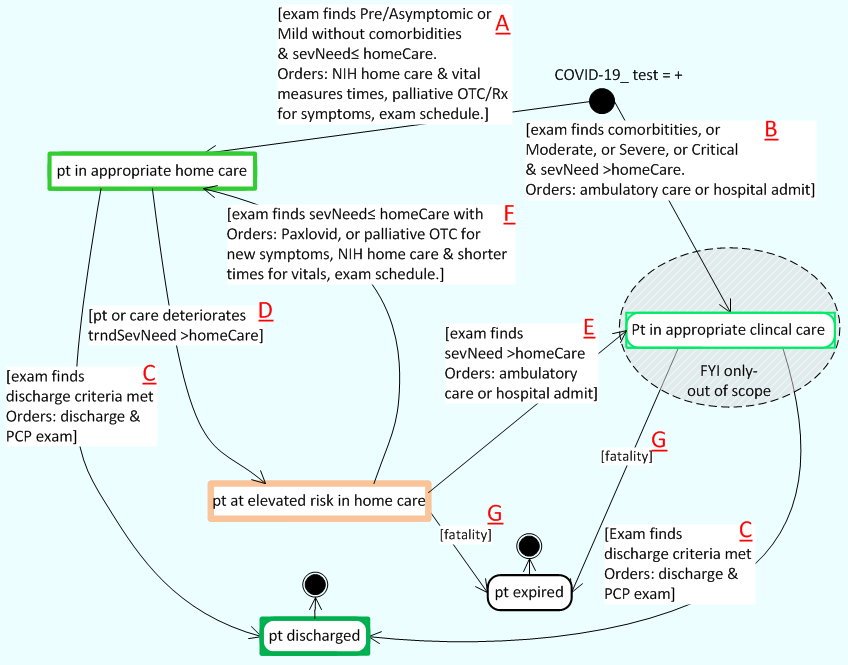
\includegraphics[scale=0.48]{cwp.png}
    \end{tabular}
  \end{center}
\caption{The \href{https://github.com/ericmercer/SPIN-bpmn-cwp-verification-paper/blob/main/26-Oct-2021-CWP.png}{CWP} for remote COVID-19 patient care.}
\label{fig:cwp}
\end{figure}